Here we shall briefly review the mathematical foundations of the AIM following closely Ref.~\cite{aim_original}. Let us suppose that exists a variable $x \in [a,b]$ where $a,b \in \mathbb{R}$ and functions $\lambda_i = \lambda_i(x) \in \mathbb{R}$ and $s_j = s_i(x) \in \mathbb{R}$ with integer indexes $i$ and $j$ that are $C_\infty(a,b)$. Let us also suppose that there is a function $y=y(x)\in\mathbb{R}$ that satisfies
%
\begin{equation}
  y^{(2)}(x) - \lambda_0(x) y^{(1)}(x) - s_0(x)y(x) = 0
  \label{eq:aim_general_ode}
\end{equation}
%
where the parenthesized superscript denotes $n$ derivatives with respect to the variable $x$. These equations can be found in many areas of physics, such as the time-independent Schr\"odinger equation in Quantum Mechanics, or the differential equations governing the perturbations of a Schwarzschild black hole. The AIM is based upon the following theorem:

\begin{theorem}
  The differential equation~\eqref{eq:aim_general_ode} has a general solution of the form
  %
  \begin{equation}
    y(x) = \exp\left( -\int^x\alpha\ud t \right) \left\{ C_2 + C_1 \int^{x} \exp \left[ \int^{t} ( \lambda_0(\tau) + 2\alpha(\tau) )\ud \tau \right] \ud t \right\}
    \label{eq:aim_general_solution}
  \end{equation}
  %
  if for some $n>0$ the condition
  %
  \begin{equation}
    \alpha(x) \equiv \frac{s_n(x)}{\lambda_n(x)} = \frac{s_{n-1}(x)}{\lambda_{n-1}(x)}
    \label{eq:aim_alpha_definition}
  \end{equation}
  %
  or equivalently
  %
  \begin{equation}
    \delta(x) \equiv s_n(x)\lambda_{n-1}(x) - \lambda_{n}(x)s_{n-1}(x) = 0
    \label{eq:aim_delta_definition}
  \end{equation}
  %
  is satisfied, where
  %
  \begin{align}
    \lambda_k(x) & \equiv \lambda^{(1)}_{k-1}(x) + s_{k-1}(x) + \lambda_0(x)\lambda_{k-1}(x) \label{eq:aim_lambda_k} \\
    s_k(x)       & \equiv       s^{(1)}_{k-1}(x) + s_0(x)\lambda_{k-1}(x) \label{eq:aim_sk}
  \end{align}
  %
  with $k \in [1, n]$
  \label{theo:aim_theorem}
\end{theorem}
%
From now on, we shall refer to the condition expressed by Eq.~\eqref{eq:aim_delta_definition} as the \emph{AIM quantization condition}. Provided that Theo.~\ref{theo:aim_theorem} is satisfied we can find both the eigenvalues and eigenvectors of Eq.~\eqref{eq:aim_general_ode} using, respectively, Eq.~\eqref{eq:aim_delta_definition} and Eq.~\eqref{eq:aim_general_solution}. More specifically, the quasinormal modes of a perturbed black hole will be the complex frequency values $\omega$ that satisfy Eq.~\eqref{eq:aim_delta_definition} for any value of $x$. Recently, it was shown in Ref.~\cite{Ismail2020} that for the method to converge, one must have
%
\begin{equation}
  \lim_{n \rightarrow \infty} \frac{\delta_n(x)}{\lambda_{n-1}^2(x)} = 0
  \label{eq:aim_convergence_criteria}
\end{equation}

Despite being quite general, the method presents a computational difficulty hidden in Eq.~\eqref{eq:aim_lambda_k} and Eq.~\eqref{eq:aim_sk}. The definitions of the $n$-th coefficients are coupled, recursive and involve the derivatives of previous entries. This means that to compute the quantization condition, Eq.~\eqref{eq:aim_delta_definition}, using $n$ iterations we end up computing the $n$-th derivatives of $\lambda_0$ and $s_0$ multiple times. Depending on the size of the original functions, the size and complexity of each coefficient can quickly spiral out of control as $n$ is increased. To address these issues, Cho et al. have proposed in Ref.~\cite{aim_improved} to instead of computing these coefficients directly, use a Taylor expansion of both $\lambda_n(x)$ and $s_n(x)$ around an arbitrary point $\xi$ where the AIM is to be performed, thus introducing a new free parameter to the method. We, however, remind the reader that the results must be independent of the choice of $\xi$. Mathematically, we have
%
\begin{align}
  \lambda_n(\xi) = & \sum_{i=0}^{\infty}c^{i}_n(x - \xi)^i, \label{eq:taylor_lambda0} \\
  s_n(\xi) =       & \sum_{i=0}^{\infty}d^{i}_n(x - \xi)^i, \label{eq:taylor_s0}
\end{align}
%
where $c^i_n$ and $d^i_n$ are the Taylor coefficients of the expansions of $\lambda_n$ and $s_n$ around $\xi$, respectively. By plugging Eqs.~\eqref{eq:taylor_lambda0} and \eqref{eq:taylor_s0} into Eqs.~\eqref{eq:aim_lambda_k} and Eq.~\eqref{eq:aim_sk} one gets

\begin{align}
  c^i_n = & (i+1)c^{i+1}_{n-1} + d^i_{n-1} + \sum_{k=0}^{i}c^k_0c^{i-k}_{n-1}, \label{eq:cin_def} \\
  d^i_n = & (i+1)d^{i+1}_{n-1} + \sum_{k=0}^{i}d^k_0c^{i-k}_{n-1}. \label{eq:din_def}
\end{align}
%
Finally, using Eqs.~\eqref{eq:cin_def} and \eqref{eq:din_def} the quantization condition, Eq.~\eqref{eq:aim_delta_definition}, becomes
%
\begin{equation}
  \delta \equiv d^0_n c^0_{n-1} - d^0_{n-1}c^0_n = 0.
  \label{eq:improved_delta}
\end{equation}

In order to better visualize and understand the improved algorithm, it is useful to arrange the $c^i_n$ (or $d^i_n$) coefficients as elements of a matrix $C$ (or $D$), where the index $i$ indicates the matrix row and the index $n$ represents the matrix column. To aid in our visualization, let us also assume, without loss of generality, that we have chose to perform the AIM with $n=2$. According to Eq.~\eqref{eq:improved_delta}, the largest $n$ coefficients that need to be computed  are $d^0_2$ and $c^0_2$. These coefficients need, in turn, to be computed recursively via Eqs.~\eqref{eq:cin_def} and \eqref{eq:din_def}. This process was represented in Fig.~\ref{fig:aim_coeffs_c} for $c^0_2$. Each row in the figure represents a step in the algorithm. A red circle marks the coefficient that is being calculated at the given step and a blue circle with arrows mark the coefficients that are necessary for the calculation. We remind that the first column of the matrices, that is, $c^i_0$ and $d^i_0$, are computed directly from $\lambda_0(x)$ and $s_0(x)$ from their Taylor expansions. Note that the lower right coefficients of the $c^i_n$ matrix, that is, $c^1_1$, $c^2_2$ and $c^2_1$ are never used in any step. Since these coefficients are not required, they need not be computed, saving time in the algorithm.

\begin{figure}[!ht]
  \centering
  \includesvg[scale = 0.75]{img/aim_qnm/aim_coeffs.svg}
  \caption{Schematic representation of the AIM for computing the $c^i_n$ matrix. Each row of matrices represent an AIM step. Coefficients circled in red are currently being computed, while coefficients marked in blue withe arrows are the coefficients required for that computation. Notice how the lower-right triangle of coefficients is never used.}
  \label{fig:aim_coeffs_c}
\end{figure}

In  Fig.~\ref{fig:aim_coeffs_d}, we see a similar representation, but now for the $d^i_n$ coefficients. The first two rows of the image represent the steps required for computing $d^0_2$. Notice however, that $d^0_1$ (the third row in the image) is not explicitly required for the computation of the target coefficients, but it is required for the computation of $c^0_2$ and can be readily calculated since it depends only on the initial Taylor expansion of the ODE coefficients. Similarly, coefficients $d^1_2$, $d^2_2$ and $d^2_1$ are never used and thus do not need to be computed.

\begin{figure}[!ht]
  \centering
  \includesvg[scale = 0.75]{img/aim_qnm/aim_coeffs_d.svg}
  \caption{Schematic representation of the AIM for computing the $d^i_n$ matrix. The first two row of matrices represent AIM steps and the third row represents the computation of $d^o_1$, which is required in computing $c^0_2$. Coefficients circled in red are currently being computed, while coefficients marked in blue withe arrows are the coefficients required for that computation. Notice how the lower-right triangle of coefficients is never used.}
  \label{fig:aim_coeffs_d}
\end{figure}

These observations motivate us to see the AIM algorithm as an ``evolution'' of the initial coefficient sets $c^i_0$ and $d^i_0$ by rewriting Eqs.~\eqref{eq:cin_def} and \eqref{eq:din_def} as
%
\begin{align}
  c^i_{n+1} = & (i+1)c^{i+1}_n + d^i_n + \sum_{k=0}^{i}c^k_0c^{i-k}_n, \label{eq:cin_iterative} \\
  d^i_{n+1} = & (i+1)d^{i+1}_n + \sum_{k=0}^{i}d^k_0c^{i-k}_n, \label{eq:din_iterative}
  .
\end{align}
%
We can now devise an algorithm that performs $n$ iterations of the AIM:
%
\begin{enumerate}
  \item Construct two arrays of size $n$ where the $i$-th element is $c^i_0$ (or $d^i_0$) where $i$ ranges from zero to $n$. We shall call these \texttt{icda} (initial $c$ data array) and \texttt{idda} (initial $d$ data array).

  \item Construct two arrays of size $n$ to contain the current column of $c$ (or $d$) indexes. We shall call these \texttt{ccda} (current $c$ data array) and \texttt{cdda} (current $d$ data array)

  \item Construct two arrays of size $n$ to contain the previous column of $c$ (or $d$) indexes. We shall call these \texttt{pcda} (previous $c$ data array) and \texttt{pdda} (previous $d$ data array).

  \item Initialize \texttt{ccda} with data from \texttt{icda} and \texttt{cdda} with data from \texttt{idda}.

  \item Perform $n$ AIM steps using the evolution Eqs.~\eqref{eq:cin_iterative} and \eqref{eq:din_iterative}. That is, repeat the following $n$ times:
        \begin{enumerate}
          \item Copy the content from \texttt{ccda} into \texttt{pcda}
          \item Copy the content from \texttt{cdda} into \texttt{pdda}
          \item Rewrite each element of \texttt{ccda} and \texttt{cdda} using Eqs. \eqref{eq:cin_iterative} and \eqref{eq:din_iterative}, respectively.
        \end{enumerate}

  \item Compute the quantization condition, Eq.~\eqref{eq:improved_delta}, using the first indexes of each array. Explicitly, perform \texttt{cdda[1]*pcda[1] - pdda[1]*ccda[1]}\footnote{We assume 1-base array indexing, the same scheme adopted by the \texttt{Julia}.}.

  \item If the coefficients are analytic, determine the roots of the resulting expression, otherwise use steps 1-6 to build a function that returns $\delta$ numerically with a given parameter set and use a numerical root finding method to find the roots of this function.
\end{enumerate}
%
The algorithm steps are depicted in Fig.~\ref{fig:arrays_steps} for the $n=2$ example. Each array is depicted as a sequence of blue (for storing $c^i_n$ coefficient) and red (for storing $d^i_n$ coefficients) squares, wherein each square is an array element. There are three columns of arrays, each representing, respectively, initial, current and previous data at various points in the algorithm. Each row indicates the algorithmic step that it represents to the left of the data arrays and which AIM step ($n$ value) a set of steps corresponds to. On step 5 (c), colored arrows indicate the data dependency of each index in the current arrays (similarly to what is depicted in Figs.~\ref{fig:aim_coeffs_c} and \ref{fig:aim_coeffs_d}). Hatches in array indexes represent data that is not evolved/computed.
%
\begin{figure}[!ht]
  \centering
  \fontsize{9}{10}\selectfont
  \includesvg[scale = 0.70]{img/aim_qnm/arrays.svg}
  \caption{Representation of AIM steps for an $n=2$ sized example. Arrays are represented by a sequence of blue (for storing $c^i_n$ coefficient) and red (for storing $d^i_n$ coefficients) squares, wherein each square is an array element. Each column represents, respectively, initial, current and previous data. Colored arrows indicate index dependencies. Hatches indicate ignored data.}
  \label{fig:arrays_steps}
\end{figure}

The implementation in \texttt{QuasinormalModes.jl} closely follows the description provided thus far, using additional coefficient arrays to enable multi-threading in the AIM core loop in a thread-safe manner. The online documentation for the package includes extensive tutorials, usage examples, and package documentation, which are available at \href{https://lucass-carneiro.github.io/QuasinormalModes.jl/stable/}{this link}. The code for the package is hosted on GitHub and can be found in Ref.~\cite{QuasinormalModesRepo}. The package is registered on the \texttt{Julia} package index and can be easily installed by following the instructions provided in the \texttt{README} of the GitHub repository.

We have developed a script to evaluate the performance and convergence characteristics of the QuasinormalModes.jl package. The script conducts a fundamental $s=l=0$ mode computation of a Schwarzschild black hole while sweeping the number of AIM iterations from $n=1$ to $n=100$. The error of the computation, the time taken to compute the result, and the number of iterations performed are measured 20 times and stored in distinct text files to enhance the statistical significance of the time measurements. The error is defined as the discrepancy between the AIM-computed value and values acquired in Ref.\cite{BertiQNMData}, which were obtained via via Leaver's continued fraction method. We present the error convergence outcomes in Fig.\ref{fig:package_error} using a logarithmic scale in the $y$ axis for both the real (black dots) and imaginary (red crosses) components of the mode as a function of the number of AIM iterations performed. Despite oscillations, an overall trend of convergence towards the reference values can be observed. We depict the average time taken for 20 repetitions as a function of the number of iterations in Fig.~\ref{fig:package_perf} using a log-log plot. It is possible to observe that the time taken increases with a power law trend as the number of AIM iterations increases.

\begin{figure}[!ht]
  \centering
  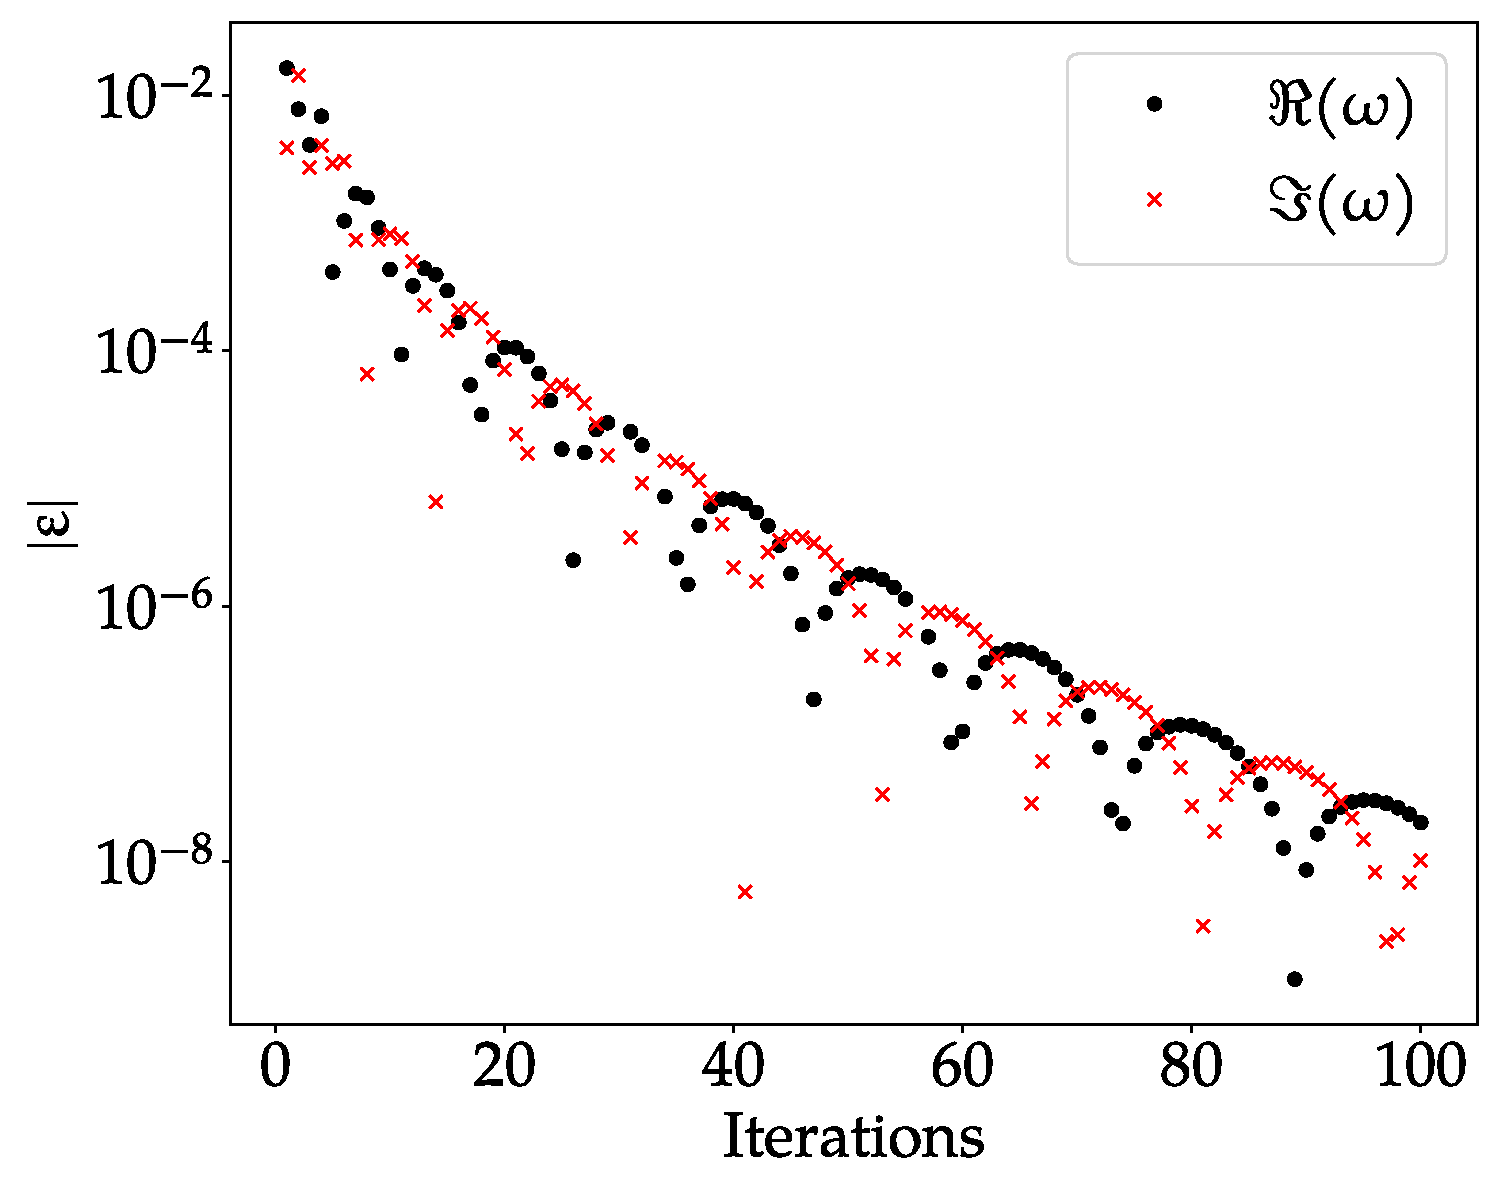
\includegraphics[width=\linewidth]{img/aim_qnm/err.pdf}
  \caption{Error of the fundamental $s=l=0$ Schwarzschild QNM vs. the number of AIM iterations. Reference values obtained in Ref.~\cite{BertiQNMData}. The y-axis of the plot is in logarithmic scale.}
  \label{fig:package_error}
\end{figure}

\begin{figure}[!ht]
  \centering
  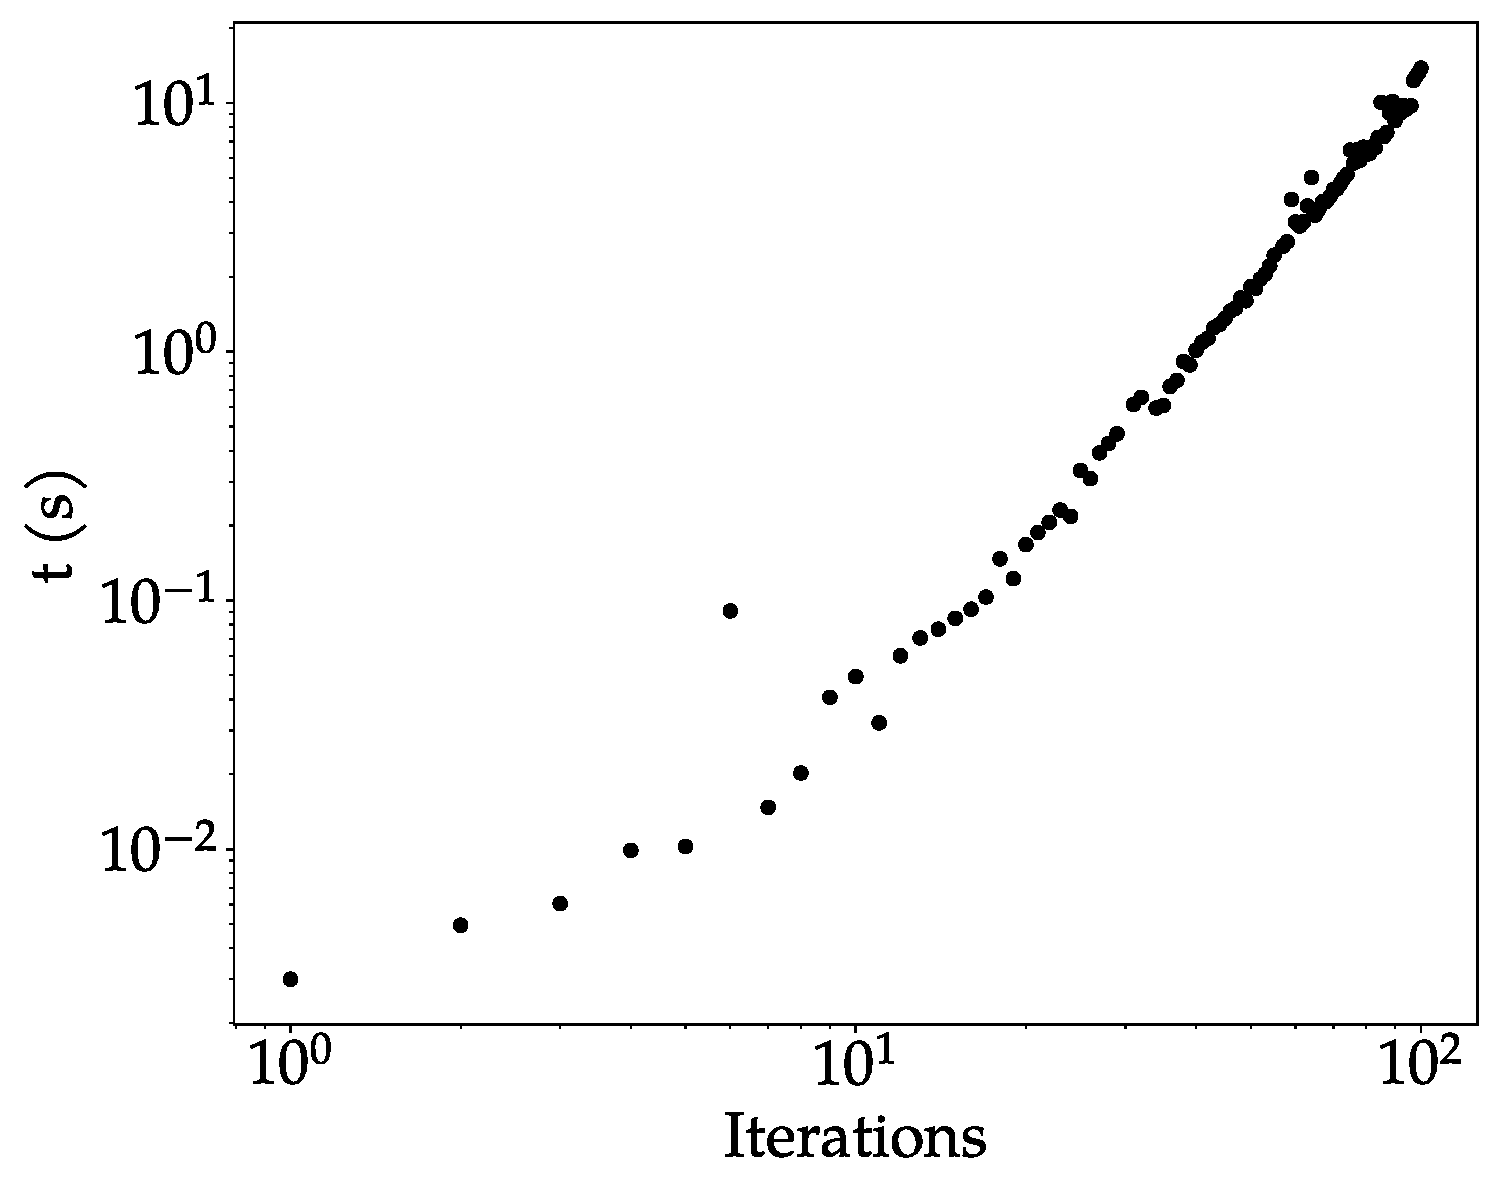
\includegraphics[width=\linewidth]{img/aim_qnm/perf.pdf}
  \caption{Time taken (average of 20 repetitions) vs. the number of AIM iterations taken to compute the fundamental Schwarzschild QNM. The plot is in a log-log scale.}
  \label{fig:package_perf}
\end{figure}